\section{Model Selection}
\subsection{Bias-Variance Tradeoff \& Sweet Spot}
\paragraph{Bias} error from \textbf{erroneous assumptions} in learning algorithm. Error can range from inaccurate assumption to simplification of model.
\paragraph{Variance} error from \textbf{sensitivity to small fluctuations} in training set.
\begin{itemize}
	\item Idea: 
	\begin{itemize}
		\item models \textbf{too simple} will have \textbf{high bias} on training data, \textbf{low variance} on test data.  $\rightarrow$ \textbf{Underfitting}
		\item models \textbf{too complex} will have \textbf{low bias} on training data, \textbf{high variance} on test data. $\rightarrow$ \textbf{Overfitting}
	\end{itemize}
	
	$\rightarrow$ find the sweet spot $\rightarrow$ \textbf{low bias \& low variance}
	
	\item \textbf{Goal} of Model Selection: \textbf{optimize} bias-variance tradeoff
	\item Criterion Metrics: \textbf{minimize} f(fitting error from given data) + g(model complexity)
	\begin{itemize}
		\item \textbf{Akaike Information Criterion(AIC)}: $AIC = -2\ln(L) + 2\cdot \#parameters$
		\item \textbf{Minimum Description Length} given the same quality: Kolmogorov Complexity
	\end{itemize}
\end{itemize}
\begin{figure}[H]
	\centering
	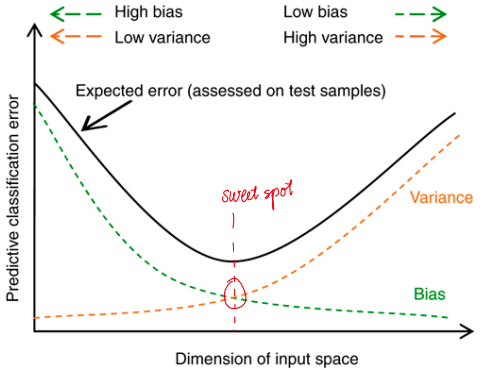
\includegraphics[width=0.5\textwidth]{bias-variance.png}
\end{figure}

\section{Evaluation}
\subsection{Evaluation Methods of Model}
\begin{itemize}
	\item Goal of evaluation: how good is the model on \textbf{new data}?
	\item Evaluation methods: how to get the \textbf{test data}?
	\begin{itemize}
		\item on training set
		\item Holdout set (stratified / repeated)
		\item k-Fold Cross-Validation (w/o stratified)
		\item Leave-One-Out Validation 
		\item Bootstrap
	\end{itemize}
\end{itemize}

\subsubsection{Evaluation Directly on Training Set: Not Preferred}
\begin{itemize}
	\item might cause \textbf{overfitting}.
	\item evaluation too optimistic, the actual error rate is higher.
\end{itemize}
$\rightarrow$ not preferred!!

\subsubsection{Evaluation using Holdout Set}
\begin{itemize}
	\item reserve data from whole data. rule of thumb: $\frac{1}{3}$ of whole.
	\item holdout set method:
	\begin{itemize}
		\item \textbf{stratified Holdout}: considers \textbf{distribution of classes}. split the training/test data \textbf{proportionally} according to the ratio of classification results. 
		\item \textbf{repeated Holdout}: \textbf{randomly} select holdout set \textbf{repeatedly} and estimate through \textbf{average error}.
	\end{itemize}
\end{itemize}

\subsubsection{Evaluation using (stratified) k-fold Cross Validation}
Process:
\begin{itemize}
	\item \textbf{partition} the data (\textbf{proportionally, if stratified}) into $k$ complementary subsets. 
	\item \textbf{train} on $(k-1)$ subsets, \textbf{test} on 1 subset.
	\item repeat until each subset is tested once.
	\item calculate the \textbf{average error rate}.
\end{itemize}

\subsubsection{Evaluation using Leave-One-Out Validation}
\begin{itemize}
	\item Use-case: when data is \textbf{scarce}.
	\item a \textbf{n-fold cross validation}: test on 1 instance, train on $(n-1)$ instances.
	\item Advantages:
	\begin{itemize}
		\item maximum use of data for training, especially when data is scarce.
		\item deterministic
	\end{itemize}
	Disadvantages:
	\begin{itemize}
		\item high computational cost
		\item non-stratified samples
	\end{itemize}
\end{itemize}

\subsubsection{Evaluation using Boostrap}
Process:
\begin{itemize}
	\item draw $n$ \textbf{random samples with replacement} as test data.
	\item test and calculate the error rate.
	\item repeat the random sampling for many times.
	\item calculate the variance/confidence interval of the sample.
\end{itemize}
Comparison to k-fold cross validation: sampling \textbf{without} replacement. 

\subsubsection{Significance between Models: Paired T-Test}
\begin{itemize}
	
	
	\item Goal: compare the \textbf{error rate} of 2 models 
	
	$\rightarrow$ see which model fits better to the \textbf{training data}
	
	$\rightarrow$ better model will predict on \textbf{test data}.
	
	\item Idea: results of a validation may be considered as \textbf{random chance}.
	
	$\rightarrow$ only \textbf{significant difference} counts! $\rightarrow$ significance test
	
\end{itemize}
\paragraph{Paired T-test: }
\subparagraph{Significantly Different? two-sided Test}
\begin{itemize}
	\item $H_0$: $\mu_d = 0$
	
	$H_1$: $\mu_d \neq 0$ 
	\item test statistic: 
	$$t = \frac{\bar{d} - \mu_d}{s_d / \sqrt{n}}$$
	\item critical value: $t_{1-\frac{\alpha}{2}, n-1}$
	\item Reject $H_0$: $|t| \geq t_{1-\frac{\alpha}{2}, n-1}$
\end{itemize}
\subparagraph{Significantly Better? one-sided Test}
\begin{itemize}
	\item $H_0$: $\mu_{C1 - C0} \leq 0$, classifier 1 is not significantly better than baseline classifier.
	
	$H_1$: $\mu_{C1 - C0} > 0$, classifier 1 is significantly better than baseline classifier
	\item critical value: $t_{1-\alpha, n-1}$
	\item Reject $H_0$: $t \geq t_{1-\alpha, n-1}$
\end{itemize}
\subsection{Quality Metrics of Model on Test Data}

\subsubsection{Confusion Matrix}
\begin{figure}[H]
	\centering
	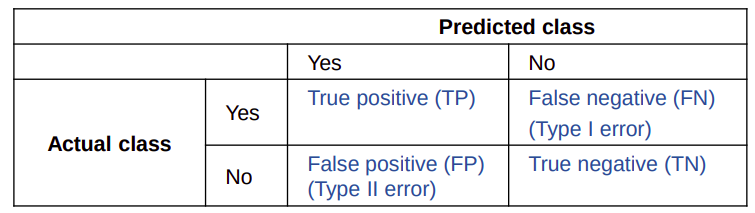
\includegraphics[width=0.65\textwidth]{confusion.png}
\end{figure}
\textbf{Overall Diagonally}:
\subparagraph{Accuracy} $$\text{Accuracy} = \frac{TP + TN}{N}$$
\subparagraph{Error Rate} $$\text{Error Rate} = 1 - \text{Accuracy} = \frac{FP + FN}{N}$$

\textbf{Specific Horizontally}:
\subparagraph{True Positive Rate / Recall / Hit Rate} $$\text{True Positive Rate/Recall} = \frac{TP}{TP + FN}$$
\subparagraph{True Negative Rate / Specificity} $$\text{True Negative Rate/Specificity} = \frac{TN}{TN + FP}$$
\subparagraph{False Positive Rate / False Alarm Rate} $$\text{False Positive Rate/False Alarm Rate} = 1- \text{Specificity} = \frac{FP}{TN + FP}$$

\textbf{Specific Vertically}:
\subparagraph{Precision} $$\text{Precision} = \frac{TP}{TP + FP}$$


\textbf{Cost-Sensitive Learning}:
\begin{itemize}
	\item Goal of general test data evaluation: minimize \textbf{overall error rate}
	
	$\rightarrow$ same weight on each prediction
	
	\item Idea in cost-sensitive learning: 
	\begin{itemize}
		\item unbalanced data
		\item prediction has different cost
	\end{itemize}
	\item Goal in cost-sensitive learning: minimize \textbf{cost}
	\item Solution:
	\begin{itemize}
		\item \textbf{weighting} of instance according to cost
		\item \textbf{resampling} of instance according to cost
		\item \textbf{predict probabilities} instead of predicting classes. minimize the cost by selecting a better \textbf{cutoff-value} (default: 0.5)
	\end{itemize}
	$\rightarrow$ the model \textbf{biased towards cost-sensitive} prediction. 
	
	$\rightarrow$ eg: in churn prediction, better predict more churns (more false positives as false negatives)
\end{itemize}


\subsubsection{Gain Curve}
\begin{itemize}
	\item Idea: visualize results of \textbf{different cutoffs}.
	
	$\rightarrow$ the \textbf{gain most of the targets} by just taking \textbf{a percentage of the whole dataset}, no need to go through the whole.
	
	$\rightarrow$ evaluate models in \textbf{cost-sensitive learning}
	\item Process:
	\begin{itemize}
		\item predict probabilities instead of classes.
		\item \textbf{sort} instances by probability \textbf{in descending order}	
	\end{itemize}
	\item x-axis: percentage of the dataset 
	\item y-axis: percentage of \textbf{actual true} instances in the whole given dataset
\end{itemize}
\begin{figure}[H]
	\centering
	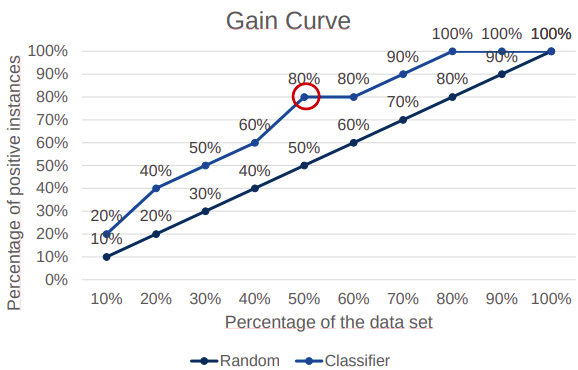
\includegraphics[width=0.55\textwidth]{gain.png}
\end{figure}
\subsubsection{Lift Curve}
\begin{itemize}
	\item Idea: visualize \textbf{how much better} sorting and taking the q\% of data set is than random sampling q\%.
	
	\item x-Axis: percentage of the dataset $q$
	\item y-Axis: Ratio of sorting and taking the q\% to random sampling 
		
	$\rightarrow$ min(Lift) = 1
		
	$$\text{Lift}(q) = \frac{\text{Gain}(q)}{q}$$

\end{itemize}
\begin{figure}[H]
	\centering
	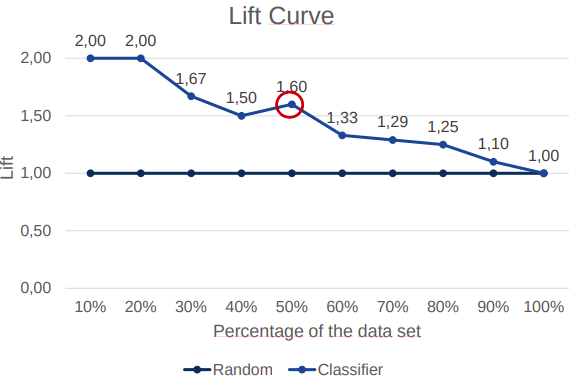
\includegraphics[width=0.55\textwidth]{lift.png}
\end{figure}
\subsubsection{ROC Curve}
\begin{itemize}
	\item Idea: go through all sizes of samples
	\item x-Axis: false positive rate
	\item y-Axis: true positive rate
	\item Process: 
	\begin{itemize}
		\item \textbf{sort} the predicted probability (the given table might be unsorted).
		\item increase the sample size \textbf{step-wise} as a cutoff for positive prediction, 
		\begin{itemize}
			\item with one more true positive (+), \textbf{go up} one step.
			\item with one more false positive(-), \textbf{go right} one step
		\end{itemize}
		 
	\end{itemize}
	\item Choosing cut-off value: choose the \textbf{percentage that bends to the left the most}.
	\item Comparing 2 models: choose the model that \textbf{bends to the left} the most.
	\item Mark the cut-off value: find the corresponding \textbf{instance predicted at cut-off value}.
\end{itemize}
\begin{figure}[H]
	\centering
	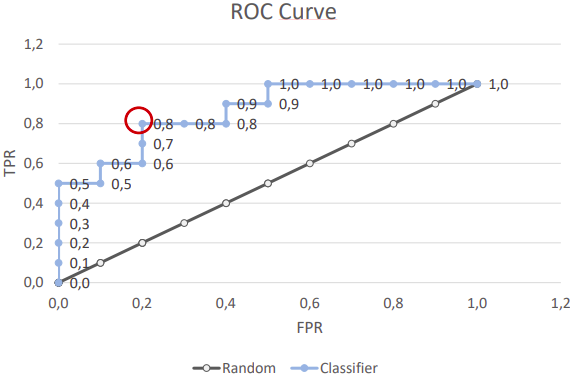
\includegraphics[width=0.55\textwidth]{roc.png}
\end{figure} 
